\section{Profiloldal és kliensoldali adatkezelés}

A profiloldal az alkalmazás azon része, ahol a felhasználó a saját filmgyűjteményét követheti. Az oldal csak bejelentkezett felhasználó számára érhető el, ezért a betöltéskor az alkalmazás lekéri a profiladatokat, a megnézett filmeket és a watchlist tartalmát. Ha bármelyik lekérdezés jogosultsági hibát ad vissza, a felhasználó a bejelentkezési oldalra kerül.

A felület felső része a profilhoz tartozó alapinformációkat jeleníti meg, például az e-mail címet és a regisztráció dátumát. A központi tartalom két fülre van bontva: az egyik a megnézett filmeket, a másik a későbbre elmentett filmeket listázza. A jobb oldali összegző rész rövid statisztikákat mutat, például a watched és watchlist elemek számát, valamint a legutóbbi aktivitás dátumát.

\begin{figure}[H]
    \centering
    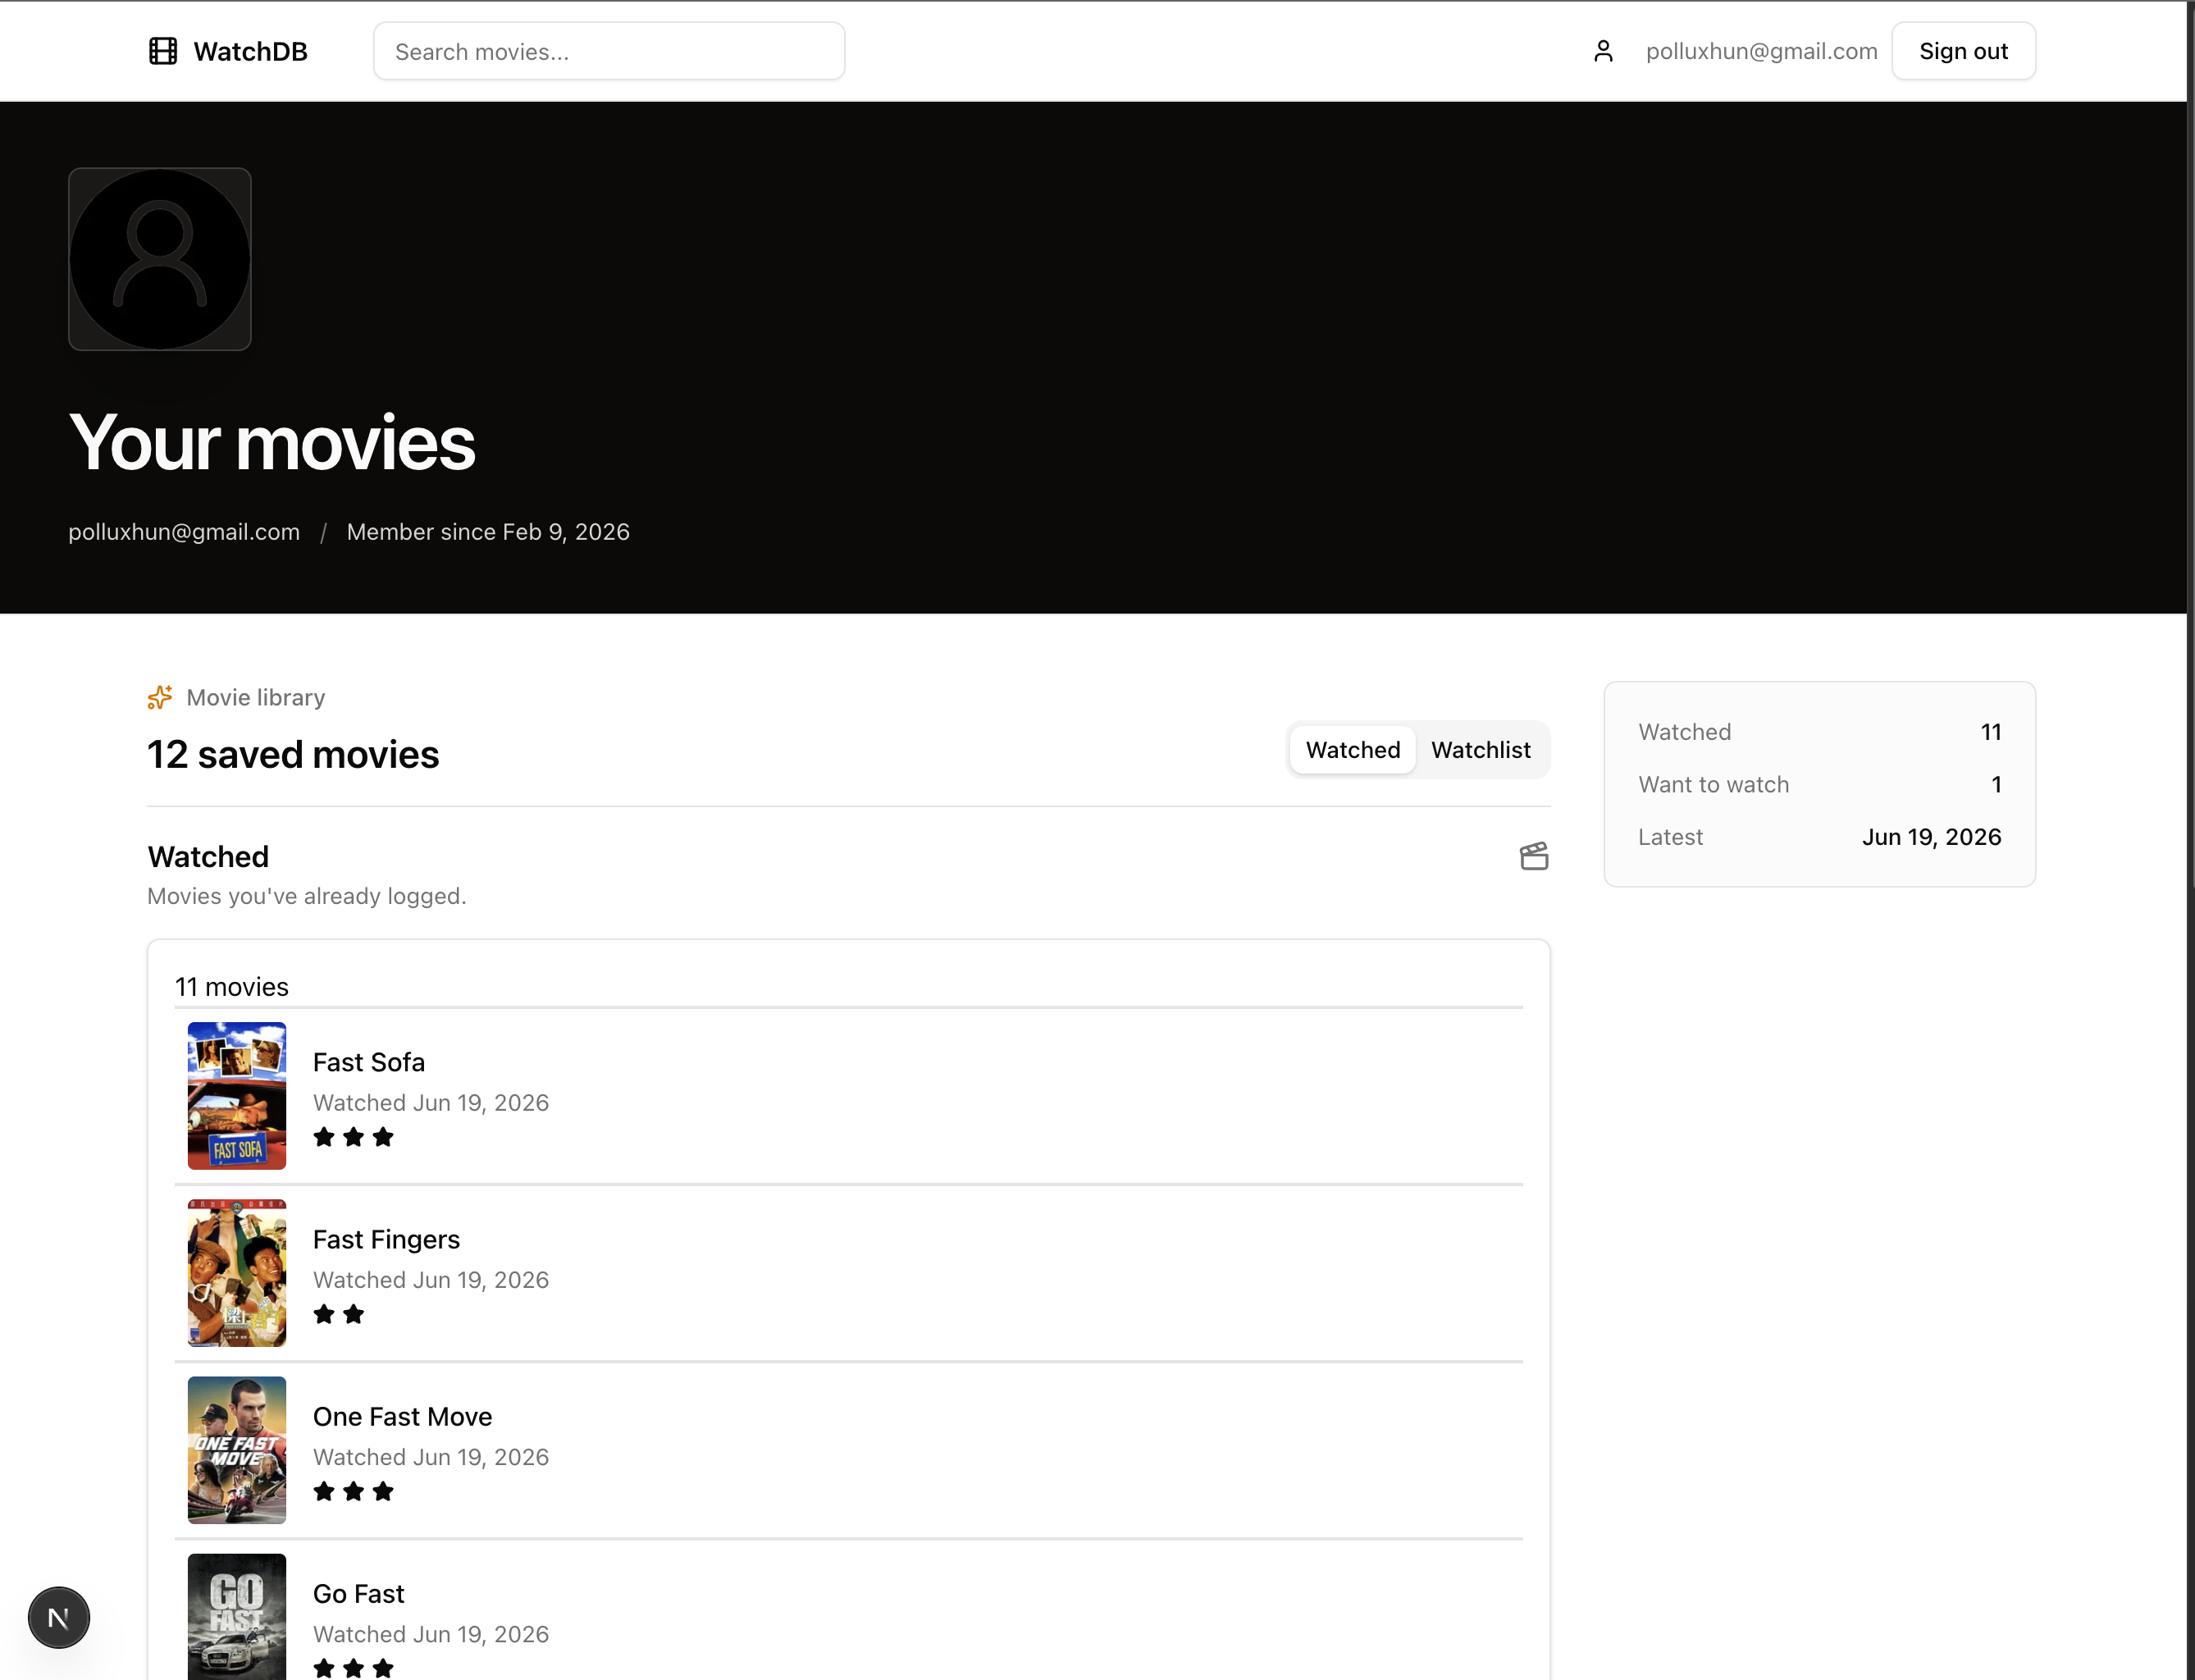
\includegraphics[width=0.82\textwidth]{chapters/chapter-6-implementation/profile-page.png}
    \caption{A profiloldal felhasználói felülete}
    \label{fig:watchdb-profile-page}
\end{figure}

A kliensoldali adatkezelést a TanStack Query biztosítja. A profiladatok, a watchlist lista és a watched lista külön query kulcsokhoz kapcsolódnak. Ez azért hasznos, mert a film oldalon végrehajtott módosítások után pontosan azok a cache-bejegyzések frissíthetők vagy érvényteleníthetők, amelyeket a profiloldal is használ.
